%----------------------------------------------------------------------------------------
%	Deep Learning
%----------------------------------------------------------------------------------------
\section{Deep Learning}

%------------------------------------------------
%Subsection: Overview
\subsection{Overview}

Explain the use cases of each type of algorithm. 

%------------------------------------------------
%Subsection: Perceptrons
\subsection{Perceptrons}

%------------------------------------------------
%Subsection: MLP: Multi-Layer Perceptrons
\subsection{MLP: Multi-Layer Perceptrons}

%------------------------------------------------
%Subsection: RBM: Restricted Boltzmann Machines
\subsection{RBM: Restricted Boltzmann Machines}

https://www.cs.toronto.edu/~hinton/absps/guideTR.pdf \\

"\textbf{Restricted Boltzmann machines (RBMs)} have been used as generative models of many different types of data including labeled or unlabeled images \cite{Hinton:2006:FLA:1161603.1161605}, windows of mel-cepstral coefficients that represent speech (Mohamed et al., 2009), bags of words that represent documents (Salakhutdinov and Hinton, 2009), and user ratings of movies (Salakhutdinov et al., 2007). In their conditional form they can be used to model high-dimensional temporal sequences such as video or motion capture data (Taylor et al., 2006) or speech (Mohamed and Hinton, 2010). Their most important use is as learning modules that are composed to form deep belief nets \cite{Hinton:2006:FLA:1161603.1161605}." \\

\begin{figure}[tb]
\centering 
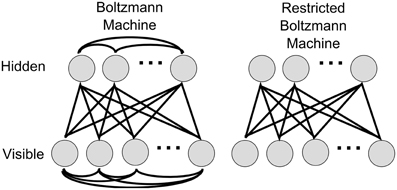
\includegraphics[width=0.5\columnwidth]{Figures/BoltzmannMachines.jpg} 
\caption[A Boltzmann Machine diagram]{An example of a generic Boltzmann Machine versus a Restricted Boltzmann Machine, from \url{http://www.frontiersin.org/files/Articles/58710/fnins-07-00178-r2/image_m/fnins-07-00178-g001.jpg}).} % The text in the square bracket is the caption for the list of figures while the text in the curly brackets is the figure caption
\label{fig:BoltzmannMachines} 
\end{figure}

A general Boltzmann machine is a network with symmetric weights fully connecting all input and hidden nodes. The details of the weights and nodes are described later in this section. A restricted Boltzmann machine separates nodes into layers and has no intra-layer connections. General Boltzmann machines, while theoretically providing a more diverse architecture, are difficult to train in practice. The difference between a general Boltzmann Machine and the Restricted Boltzmann Machine is illustrated in Figure \ref{fig:BoltzmannMachines}. \\

The training procedure for RBMs is more complicated than back-propagation. They typically use a procedure called constrastive divergence \cite{Hinton:2002:TPE:639729.639730}. There are several meta-parameters including learning rate, momentum, weight-cost, sparsity target, initial weights, number of hidden units, and mini-batch sizes. \\

For simplicity, the outline below will consider a two-layer network consisting of the visible unit layer representing the input data and a layer of hidden units called \textbf{feature detectors}. Deep neural networks can be trained by successively stacking RBMs, with the hidden layer of the first RBM used as an input for the second. Greedy pairwise training of layers has been demonstrated to be effective in learning deep architectures (reference greedy pair training). Input data are stochastic binary pixels (or continuous variables scaled to $[0,1]$). Feature detectors are also stochastic binary units. The visible units are connected to the feature detectors using symmetrtically weighted connections. A configuration of visible and hidden units has an energy (Hopfield, 1982) given by:

\begin{equation}
E(\textbf{v},\textbf{h}) = - \sum_{i} a_{i} v_{i} -\sum_{j} b_{j} h_{j} - \sum_{i}\sum_{j}v_{i}h_{i}w_{ij}
\end{equation}

for $i \in visible$ and $j \in hidden$. In this equation, $v_{i}$ and $h_{j}$ are the binary states of the visible unit $i$ and hidden unit $j$, respectively. $a_{i}$ and $b_{j}$ are their biases and $w_{ij}$ is the weight between them. 

The energy can be used to define a probability of this pairing of visible and hidden units (hence the name "Boltzmann Machine":

\begin{equation}
p(\textbf{v},\textbf{h}) = \frac{1}{\mathcal{Z}} e^{-E(\textbf{v},\textbf{h})}
\end{equation}

Z is the partition function:

\begin{equation}
\mathcal{Z} = \sum_{\textbf{v},\textbf{h}} e^{-E(\textbf{v},\textbf{h})}
\end{equation}

The network assigns a probability to a visible vector $\textbf{v}$, which can be calculated by summing $p(\textbf{v},\textbf{h})$ over all possible hidden vectors:

\begin{equation}
p(\textbf{v}) = \frac{1}{\mathcal{Z}} \sum_{\textbf{h}} e^{-E(\textbf{v},\textbf{h})}
\end{equation}

A higher energy input is a less-probable input, according to the energy function. The network is trained to increase the probability (lowering the energy) assigned by the network to signal inputs while lowering the probability (increasing the energy) assigned to noise. To get the change in weights:

\begin{equation}
\frac{\delta \log p(\textbf{v})}{\delta w_{ij}} = \langle v_{i} h_{j} \rangle_{data} - \langle v_{i} h_{j} \rangle_{model}
\end{equation}

The angle brackets denote expectation values under the specified distribution (data or model). A learning rule for weights using stochastic gradient ascent on the log probability, and a learning rate $\epsilon$, is then simply:

\begin{equation}
\delta w_{ij} = \epsilon ( \langle v_{i} h_{j} \rangle_{data} - \langle v_{i} h_{j} \rangle_{model} ).
\end{equation}

Now all that remains is to get an unbiased sample of $\langle v_{i} h_{j} \rangle_{data}$ and $\langle v_{i} h_{j} \rangle_{model}$. The first one is straightforward, since there are no connections between hidden units of the same layer in an RBM. Given a randomly selected training image, $\textbf{v}$, the binary state, $h_{j}$ , of each hidden unit, j, is set to 1 with probability 

\begin{equation}
p(h_{j}=1 | \textbf{v}) = \sigma ( b_{j} + \sum_{i} v_{i} w_{ij} )
\end{equation}

% Resume in change of weights derivation
%------------------------------------------------
%Subsection: CNN: Convolutional Neural Networks
\subsection{CNN: Convolutional Neural Networks}

%------------------------------------------------
%Subsection: RNN: Recurrent Neural Networks
\subsection{RNN: Recurrent Neural Networks}

%------------------------------------------------
%Subsection: LSTM: Long Short Term Memory
\subsection{LSTM: Long Short Term Memory}

%------------------------------------------------
%Subsection: Auto-Encoders and Deep Belief Networks
\subsection{Auto-Encoders and Deep Belief Networks}

%------------------------------------------------
%Subsection: Neural Turing Machines
\subsection{Neural Turing Machines}
